\documentclass[times, utf8, seminar, numeric]{fer}

\usepackage{booktabs}
\usepackage{hyperref}
\usepackage{enumitem}
\usepackage{mathtools}
\usepackage{listings}
\usepackage{multirow}
\usepackage{tikz}
\usepackage{svg}
\usepackage{listings}

\definecolor{dkgreen}{rgb}{0,0.6,0}
\definecolor{gray}{rgb}{0.5,0.5,0.5}
\definecolor{mauve}{rgb}{0.58,0,0.82}

% ovo su postavke za kod
\lstset{frame=tb,
  language=Java,
  aboveskip=3mm,
  belowskip=3mm,
  showstringspaces=false,
  columns=flexible,
  basicstyle={\small\ttfamily},
  numbers=left,
  numberstyle=\tiny\color{gray},
  keywordstyle=\color{blue},
  commentstyle=\color{dkgreen},
  stringstyle=\color{mauve},
  breaklines=true,
  breakatwhitespace=true,
  tabsize=3
}

\renewcommand{\lstlistingname}{Isječak koda}% Listing -> Isječak koda

\begin{document}

\title{Izgradnja binarnog stabla valića kao RRR strukture}
\author{Mislav Magerl, Matija Milišić, Mateo Šimonović}
\voditelj{izv. prof. dr. sc. Mile Šikić}

\maketitle

\tableofcontents

\chapter{Uvod}
alo

\chapter{Stablo valića}
\begin{figure}[ht]
	\centering
	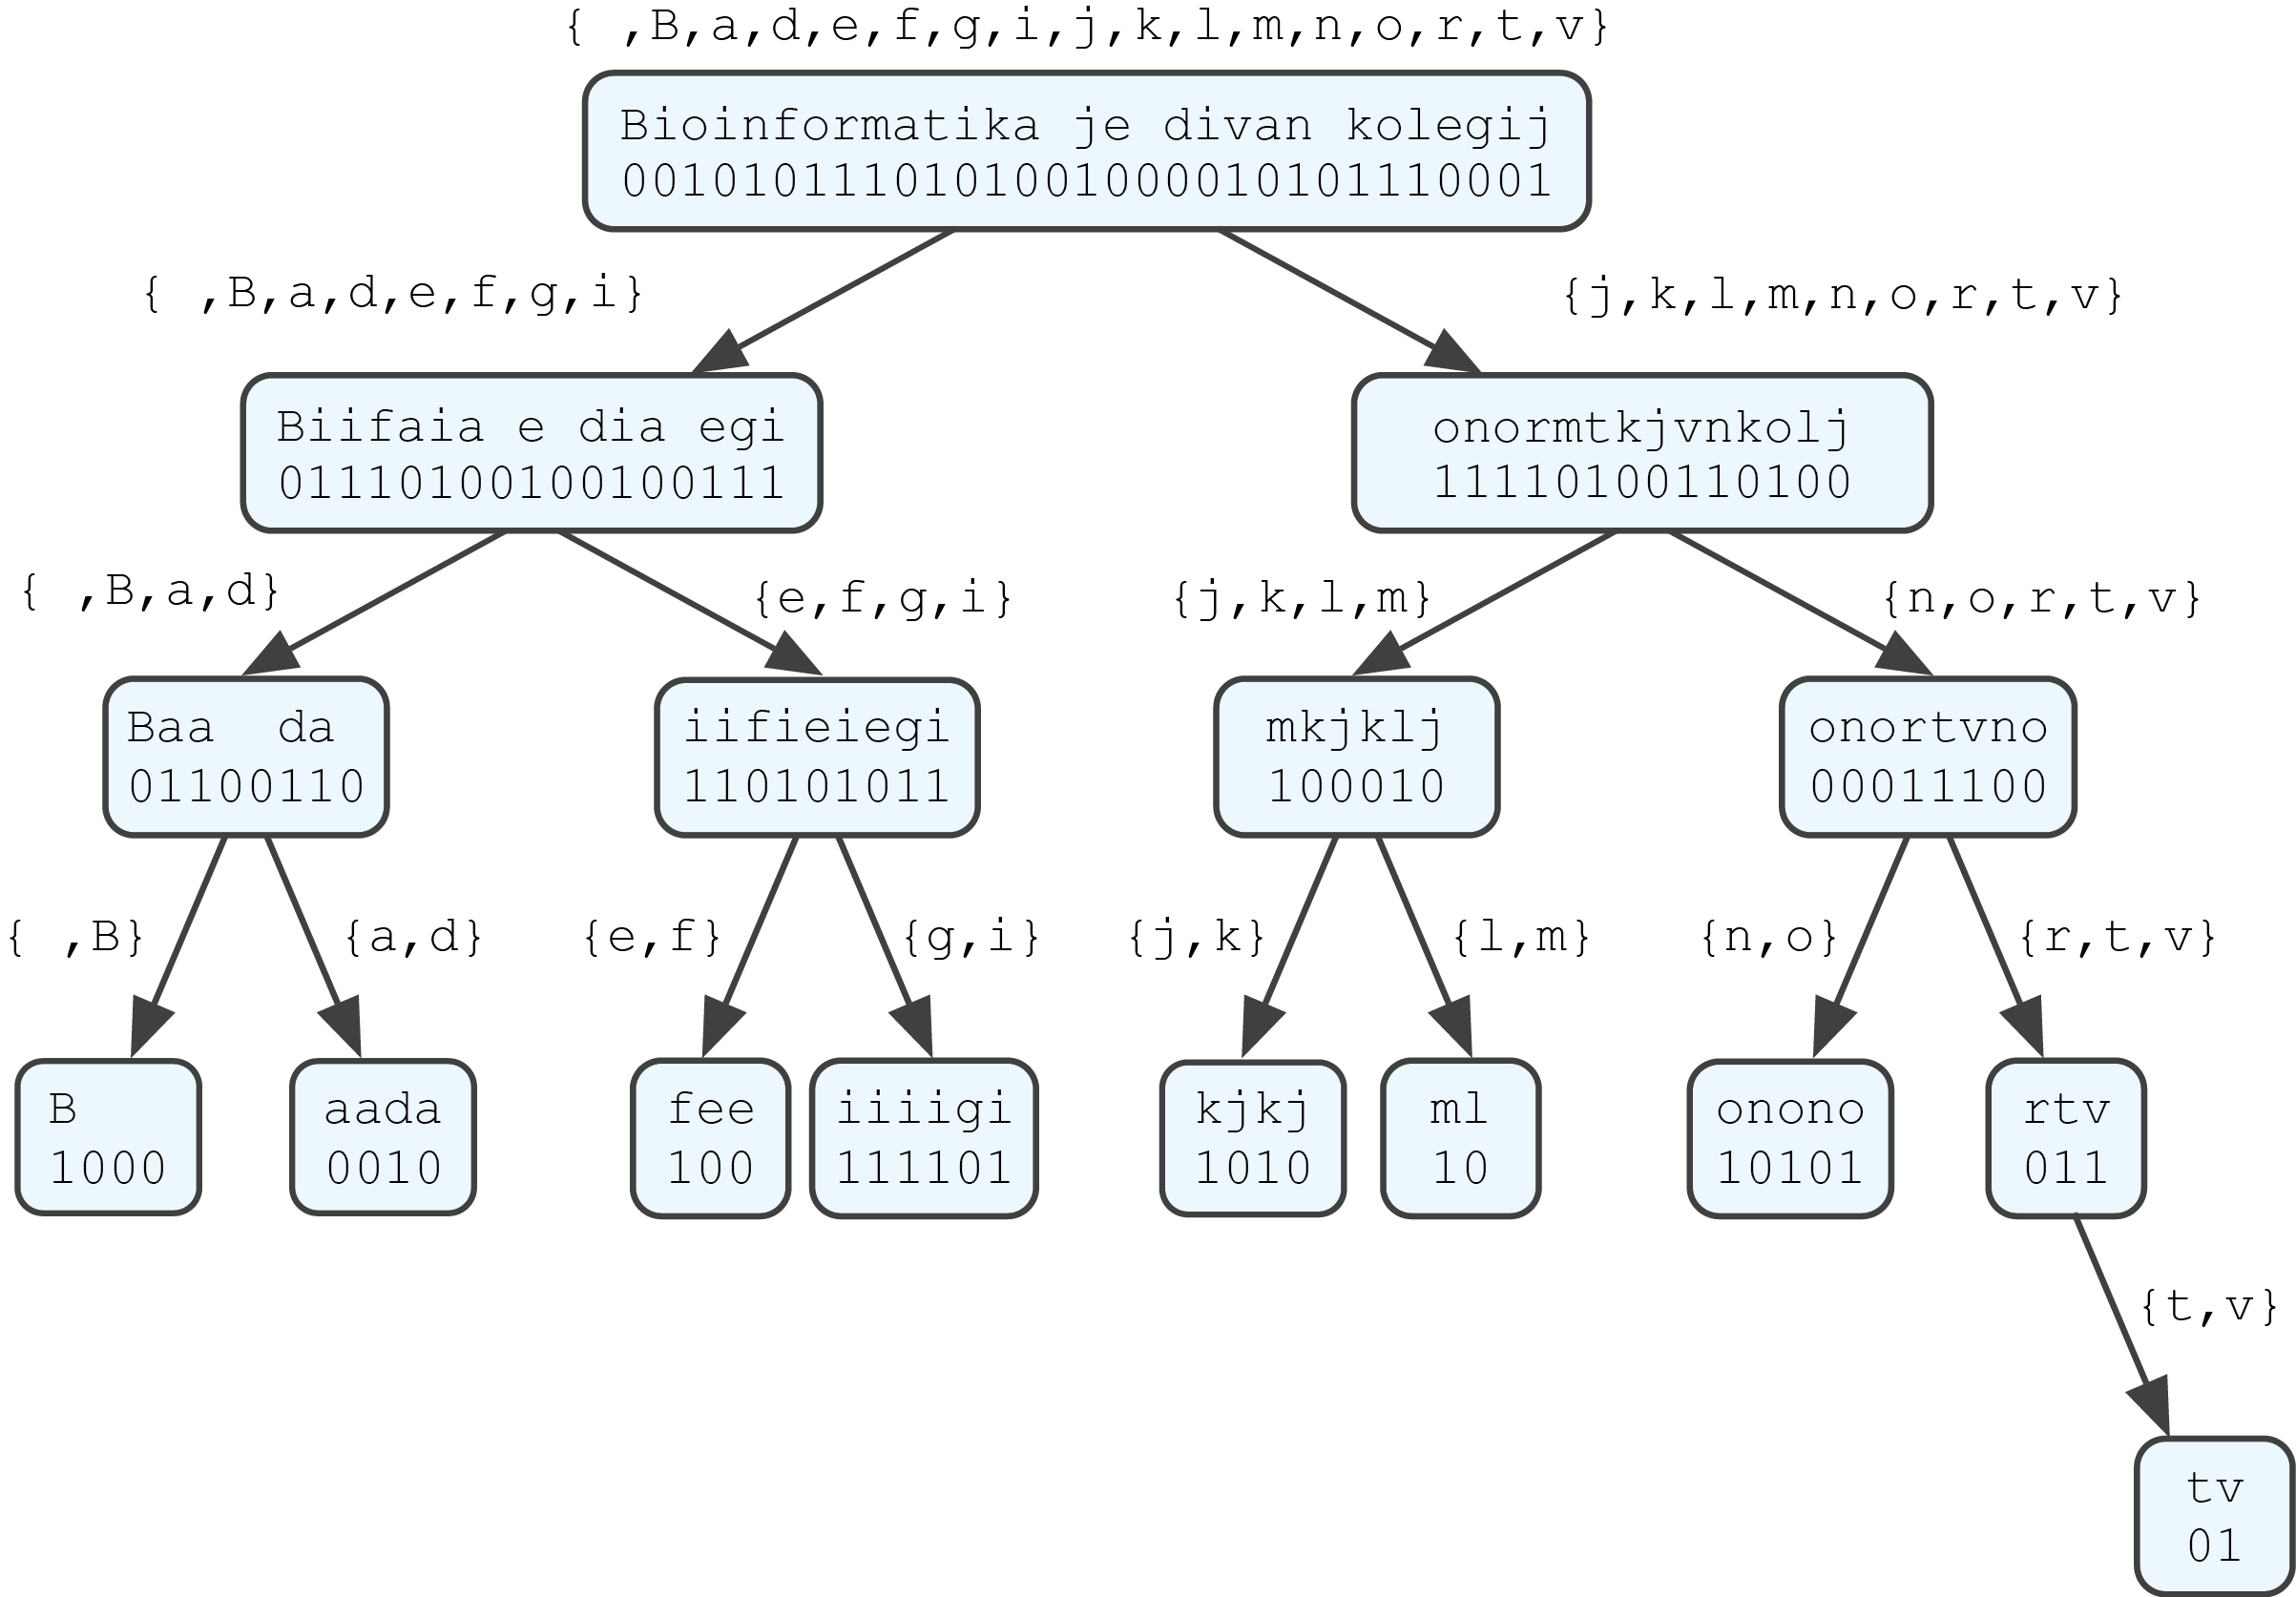
\includegraphics[width=\textwidth]{img/wavelet_tree_example.png}
	\caption{Stablo valića za ulazni niz "Bioinformatika je divan kolegij"}
	\label{fig:wavelet-tree-example}
\end{figure}

\chapter{RRR struktura}
\begin{figure}[ht]
	\centering
	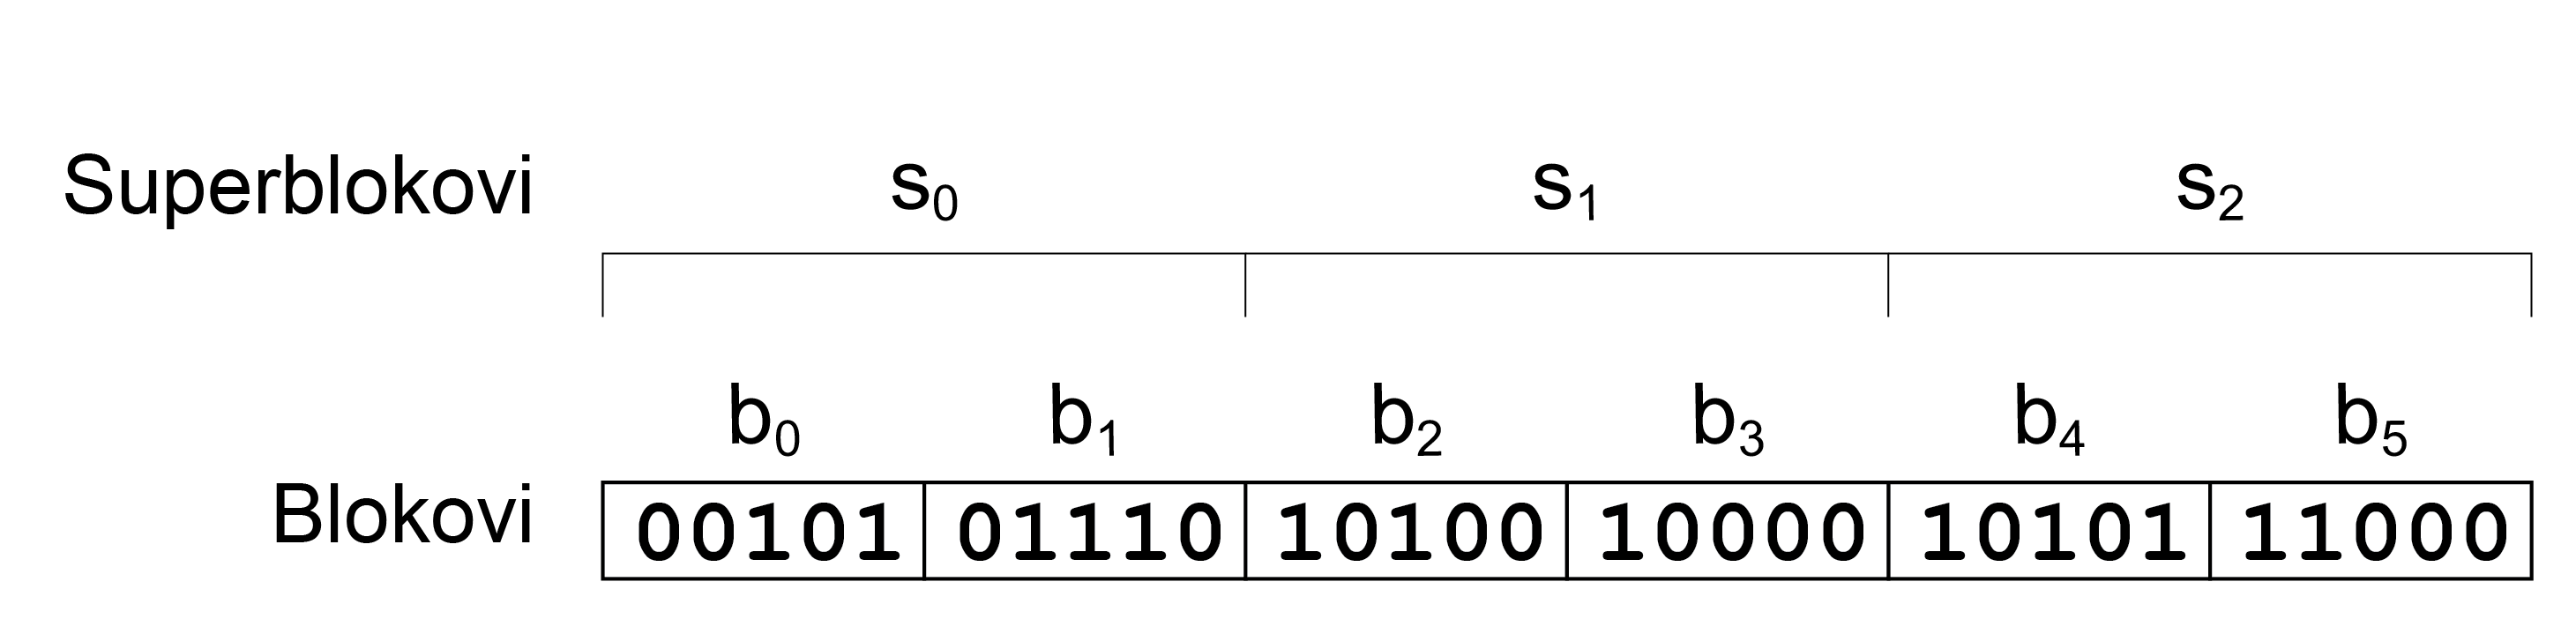
\includegraphics[width=\textwidth]{img/rrr_blocks.png}
	\caption{Prikaz blokova i superblokova RRR strukture}
	\label{fig:rrr-blocks}
\end{figure}

\bibliography{literature}
\bibliographystyle{fer}

\begin{sazetak}
Sazetak rada

\kljucnerijeci{Velvet}
\end{sazetak}

\end{document}
